\section{TỔNG QUAN ĐỀ TÀI}

\subsection{Bố cục báo cáo}
Nội dung báo cáo được trình bày trong năm chương như sau:
\begin{itemize}
    \item Chương 1: Tổng quan đề tài. Trình bày lý do chọn đề tài, mục tiêu nghiên cứu, đối tượng và phạm vi nghiên cứu, phương pháp nghiên cứu, ý nghĩa thực tiễn và bố cục của báo cáo.
    \item Chương 2: Cơ sở lý thuyết. Giới thiệu các kiến thức nền tảng liên quan đến Cloud Computing, Private Cloud, Software Defined Networking (SDN), OpenFlow, SDN Controller, VLAN, VPN/GRE Tunnel và các công nghệ được sử dụng trong đề tài.
    \item Chương 3: Phân tích và thiết kế hệ thống. Phân tích yêu cầu hệ thống, thiết kế mô hình mạng doanh nghiệp, kiến trúc Cloud, SDN, cơ sở dữ liệu và giao diện Web quản lý.
    \item Chương 4: Triển khai hệ thống và đánh giá. Trình bày quá trình triển khai các thành phần của hệ thống, xây dựng Website quản lý, thực hiện các kịch bản kiểm thử và đánh giá hiệu năng dựa trên các tiêu chí đã đề ra.
    \item Chương 5: Kết luận và hướng phát triển. Tổng kết các kết quả đạt được, đánh giá hạn chế và đề xuất hướng phát triển trong tương lai.
\end{itemize}

\subsection{Lý do chọn đề tài}
Hiện nay, có rất nhiều doanh nghiệp sở hữu mô hình gồm một trụ sở chính và nhiều chi nhánh phân bố ở các khu vực khác nhau. Điều này làm cho việc quản lý, cấu hình và giám sát hệ thống mạng của doanh nghiệp trở nên phức tạp hơn. Mô hình mạng truyền thống và cách quản trị cũ khiến doanh nghiệp gặp nhiều khó khăn trong việc đồng bộ cấu hình từng thiết bị, quản lý tập trung và giám sát tình trạng hoạt động của hệ thống mạng.

\subsubsection{Phân tích các mô hình mạng truyền thống}

\paragraph{Mô hình mạng phẳng (Flat Network)}
Mạng phẳng là kiến trúc mạng đơn giản nhất, trong đó tất cả các thiết bị được kết nối trong cùng một broadcast domain, không có sự phân chia theo các tầng hoặc vùng mạng.

\begin{figure}[H]
    \centering
    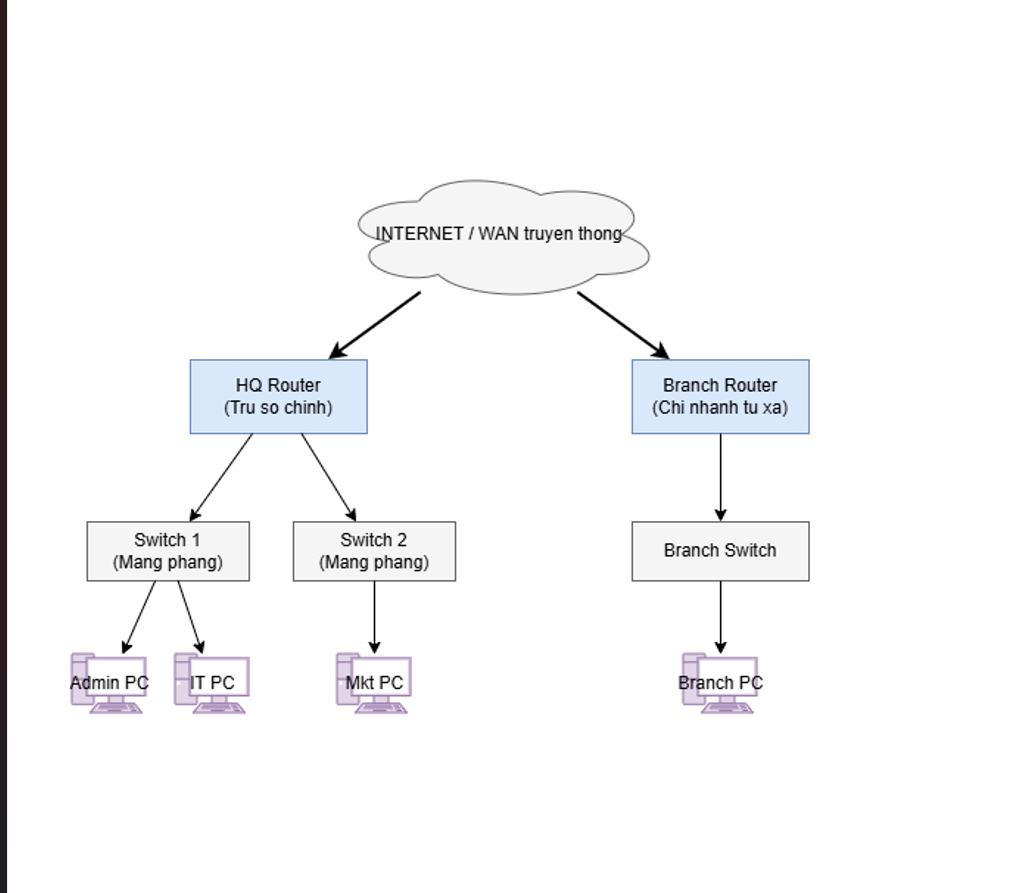
\includegraphics[width=0.8\textwidth]{image/flat_network.png}
    \caption{Sơ đồ mô hình mạng phẳng}
    \label{fig:flat_network}
\end{figure}

\textbf{Đặc điểm:}
\begin{itemize}
    \item Tất cả thiết bị nằm trong cùng một subnet và VLAN
    \item Không có sự phân cấp giữa các thiết bị mạng
    \item Broadcast traffic được truyền đến toàn bộ mạng
    \item Cấu hình đơn giản, chi phí thấp
\end{itemize}

\textbf{Khó khăn và hạn chế:}
\begin{itemize}
    \item \textbf{Hiệu năng kém:} Khi số lượng thiết bị tăng lên, broadcast storm gây quá tải mạng, làm giảm băng thông khả dụng và tăng độ trễ. Mỗi broadcast packet được gửi đến tất cả thiết bị, gây lãng phí tài nguyên mạng.
    \item \textbf{Bảo mật yếu:} Không có sự phân đoạn mạng, tất cả thiết bị có thể giao tiếp trực tiếp với nhau, khó kiểm soát truy cập và dễ bị tấn công lan truyền. Một thiết bị bị nhiễm mã độc có thể nhanh chóng lây lan sang toàn bộ mạng.
    \item \textbf{Khó quản lý:} Khi mạng mở rộng, việc theo dõi và xử lý sự cố trở nên phức tạp, không thể áp dụng chính sách khác nhau cho từng nhóm người dùng. Không có sự phân tách logic giữa các phòng ban.
    \item \textbf{Không có khả năng mở rộng:} Giới hạn về số lượng thiết bị do broadcast domain lớn, không phù hợp với doanh nghiệp có nhiều phòng ban hoặc chi nhánh. Broadcast domain càng lớn, hiệu năng càng giảm.
    \item \textbf{Thiếu tính linh hoạt:} Khó triển khai Quality of Service (QoS), không thể ưu tiên lưu lượng theo ứng dụng hoặc người dùng. Không thể áp dụng chính sách bảo mật khác nhau cho các loại traffic khác nhau.
    \item \textbf{Khó fault isolation:} Khi có sự cố xảy ra, khó xác định vị trí và phạm vi ảnh hưởng do tất cả thiết bị nằm trong cùng một domain.
    \item \textbf{Hạn chế về scalability:} Không thể mở rộng lên hàng trăm hoặc hàng ngàn thiết bị mà vẫn duy trì hiệu năng ổn định.
\end{itemize}

\paragraph{Mô hình mạng phân tầng 3 lớp (Three-Tier Hierarchical Model)}
Mô hình mạng 3 lớp là kiến trúc được thiết kế theo nguyên tắc phân cấp, chia mạng thành ba lớp: Core Layer, Distribution Layer và Access Layer, mỗi lớp có vai trò và chức năng riêng biệt.

\begin{figure}[H]
    \centering
    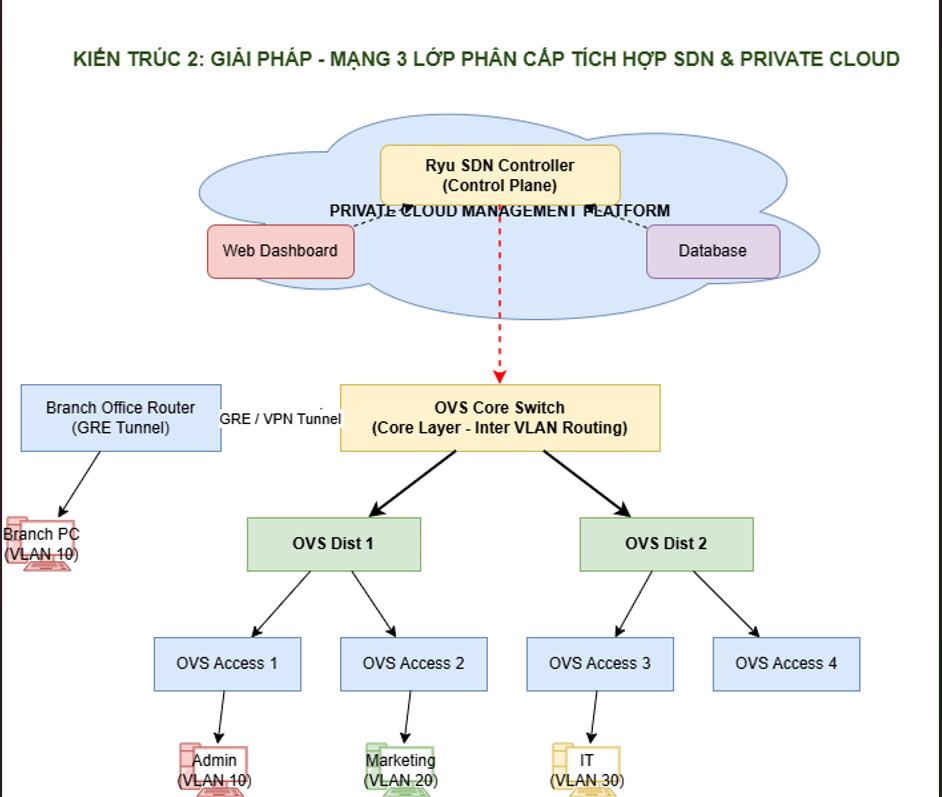
\includegraphics[width=0.8\textwidth]{image/3tier_network.png}
    \caption{Sơ đồ mô hình mạng phân tầng 3 lớp}
    \label{fig:three_tier_network}
\end{figure}

\textbf{Đặc điểm:}
\begin{itemize}
    \item \textbf{Core Layer (Lớp lõi):} Backbone của mạng, đảm nhận việc chuyển tiếp dữ liệu tốc độ cao giữa các Distribution Layer, sử dụng thiết bị hiệu năng cao, không thực hiện xử lý phức tạp
    \item \textbf{Distribution Layer (Lớp phân phối):} Nằm giữa Core và Access Layer, thực hiện routing, filtering, QoS, aggregation, áp dụng các policy và access control list (ACL)
    \item \textbf{Access Layer (Lớp truy cập):} Kết nối trực tiếp với thiết bị đầu cuối (PC, server, IP phone), thực hiện VLAN assignment, port security, 802.1X authentication
\end{itemize}

\textbf{Khó khăn và hạn chế:}
\begin{itemize}
    \item \textbf{Chi phí cao:} Cần đầu tư nhiều thiết bị phần cứng cho từng lớp (Core Switch, Distribution Switch, Access Switch), thiết bị Core và Distribution thường có giá thành rất cao. Cần phải đầu tư thiết bị dự phòng cho tính sẵn sàng cao (High Availability).
    \item \textbf{Cấu hình phức tạp:} Phải cấu hình thủ công từng thiết bị qua CLI (Command Line Interface), dễ xảy ra sai sót và không đồng nhất giữa các thiết bị. Mỗi thay đổi cấu hình đều cần can thiệp trực tiếp vào từng thiết bị.
    \item \textbf{Khó mở rộng:} Khi thêm chi nhánh mới, phải cấu hình lại nhiều thiết bị, thiết lập VPN/Tunnel, đồng bộ routing table, mất nhiều thời gian và công sức. Không có cơ chế tự động hóa để thêm thiết bị mới.
    \item \textbf{Thiếu tính linh hoạt:} Khó thay đổi topology hoặc policy khi có yêu cầu mới, phải can thiệp trực tiếp vào từng thiết bị, có thể gây gián đoạn dịch vụ. Mỗi thay đổi cần có thời gian downtime.
    \item \textbf{Quản lý phân tán:} Không có điểm quản lý tập trung, phải truy cập từng thiết bị để giám sát, backup config, update firmware. Không có cái nhìn tổng thể về toàn bộ hệ thống mạng.
    \item \textbf{Khó tự động hóa:} Việc triển khai tự động (auto-provisioning, zero-touch deployment) rất khó thực hiện với kiến trúc truyền thống. Không có API để tự động hóa các tác vụ quản trị.
    \item \textbf{Khó troubleshooting:} Khi có sự cố, phải kiểm tra từng thiết bị để tìm nguyên nhân, không có cái nhìn tổng thể về toàn bộ mạng. Không có công cụ giám sát tập trung.
    \item \textbf{Single point of failure:} Mỗi lớp có thể trở thành điểm yếu đơn lẻ, đặc biệt là Core Layer. Nếu Core Switch bị lỗi, toàn bộ mạng có thể bị ảnh hưởng.
    \item \textbf{Khả năng phản ứng chậm:} Khi có yêu cầu thay đổi nhanh từ doanh nghiệp, mạng truyền thống không thể đáp ứng kịp thời do quy trình thay đổi phức tạp.
\end{itemize}

\paragraph{So sánh tổng quan hai mô hình mạng}

\begin{table}[H]
\centering
\caption{So sánh mô hình mạng phẳng và mô hình 3 tầng}
\label{tab:network_comparison}
\begin{tabular}{|p{4cm}|p{6cm}|p{6cm}|}
\hline
\textbf{Tiêu chí} & \textbf{Mạng phẳng} & \textbf{Mạng 3 tầng} \\
\hline
\textbf{Chi phí đầu tư} & Thấp (ít thiết bị, cấu hình đơn giản) & Cao (nhiều thiết bị chuyên dụng, cấu hình phức tạp) \\
\hline
\textbf{Hiệu năng} & Kém khi số lượng thiết bị lớn (broadcast storm) & Tốt với traffic phân tầng và phân đoạn hợp lý \\
\hline
\textbf{Bảo mật} & Yếu (không có segmentation) & Tốt hơn (có segmentation và ACL) nhưng vẫn hạn chế \\
\hline
\textbf{Khả năng mở rộng} & Hạn chế (giới hạn broadcast domain) & Tốt hơn nhưng phức tạp và tốn kém \\
\hline
\textbf{Quản lý} & Đơn giản nhưng không hiệu quả khi mở rộng & Phức tạp, cần nhiều kiến thức chuyên môn \\
\hline
\textbf{Tự động hóa} & Không hỗ trợ & Khó khăn, không có cơ chế API chuẩn \\
\hline
\textbf{Phù hợp} & Mạng nhỏ, ít thiết bị (<50) & Doanh nghiệp vừa và lớn, nhiều phòng ban \\
\hline
\end{tabular}
\end{table}

\subsubsection{Giải pháp với SDN và Cloud}
Sự phát triển của công nghệ Cloud Computing và Software Defined Networking (SDN) đã mở ra hướng mới trong việc quản lý hạ tầng mạng. Cloud Computing cung cấp môi trường triển khai linh hoạt, dễ mở rộng và tối ưu chi phí đầu tư, trong khi SDN tách biệt mặt phẳng điều khiển (Control Plane) khỏi mặt phẳng chuyển tiếp dữ liệu (Data Plane), cho phép quản lý tập trung toàn bộ thiết bị mạng thông qua một bộ điều khiển (SDN Controller).

\textbf{Lợi ích của giải pháp SDN kết hợp Cloud:}
\begin{itemize}
    \item \textbf{Quản lý tập trung:} SDN Controller cung cấp single point of management cho toàn bộ mạng, có cái nhìn tổng thể về topology, traffic, và trạng thái thiết bị
    \item \textbf{Tự động hóa:} Việc cấu hình VLAN, thiết lập Flow Rule, điều khiển lưu lượng và triển khai thiết bị mới có thể được thực hiện tự động, nhanh chóng và nhất quán thông qua API
    \item \textbf{Linh hoạt:} Dễ dàng thay đổi policy, routing, QoS bằng cách cập nhật logic trên Controller mà không cần can thiệp vào từng thiết bị
    \item \textbf{Khả năng lập trình:} Sử dụng các ngôn ngữ lập trình cấp cao (Python, Java) để xây dựng các ứng dụng mạng tùy chỉnh
    \item \textbf{Giảm chi phí:} Sử dụng Open vSwitch và commodity hardware thay vì thiết bị proprietary đắt tiền
    \item \textbf{Dễ mở rộng:} Khi thêm chi nhánh hoặc thiết bị mới, Controller tự động phát hiện và cấu hình, giảm đáng kể thời gian deployment
    \item \textbf{Giám sát real-time:} Cung cấp dashboard trực quan để theo dõi bandwidth, latency, packet loss, topology changes
\end{itemize}

Xuất phát từ những yêu cầu thực tế trên, nhóm chọn đề tài "Quản lý mạng doanh nghiệp trên nền tảng Cloud sử dụng SDN" nhằm nghiên cứu và xây dựng một mô hình quản lý mạng doanh nghiệp hiện đại, góp phần nâng cao hiệu quả quản trị mạng, giảm thời gian triển khai thiết bị, tăng khả năng mở rộng và đáp ứng xu hướng phát triển của các doanh nghiệp

\subsection{Mục tiêu thực hiện đề tài}
Đề tài hướng đến việc nghiên cứu, thiết kế và triển khai mô hình quản lý mạng doanh nghiệp trên nền tảng Cloud kết hợp với công nghệ Software Defined Networking (SDN), nhằm nâng cao hiệu quả quản trị và tự động hóa quá trình vận hành hệ thống mạng.

\subsection{Đối tượng và phạm vi nghiên cứu}

\subsubsection{Đối tượng nghiên cứu}
Đối tượng nghiên cứu của đề tài bao gồm:
\begin{itemize}
    \item \textbf{Công nghệ Cloud Computing:} Nghiên cứu mô hình Private Cloud để triển khai hạ tầng ảo hóa phục vụ quản lý mạng doanh nghiệp.
    \item \textbf{Công nghệ Software Defined Networking (SDN):} Nghiên cứu kiến trúc SDN, giao thức OpenFlow, SDN Controller (Ryu Framework) và cơ chế quản lý tập trung thiết bị mạng.
    \item \textbf{Công nghệ VLAN:} Nghiên cứu phân đoạn mạng, chuẩn IEEE 802.1Q, Access Port, Trunk Port và Inter-VLAN Routing.
    \item \textbf{Công nghệ VPN/GRE Tunnel:} Nghiên cứu kết nối các chi nhánh từ xa qua mạng công cộng.
    \item \textbf{Hệ thống quản lý:} Nghiên cứu thiết kế và xây dựng giao diện Web để quản lý, giám sát và cấu hình tự động hệ thống mạng.
\end{itemize}

\subsubsection{Phạm vi nghiên cứu}
Đề tài tập trung vào các nội dung sau:
\begin{itemize}
    \item Thiết kế mô hình mạng doanh nghiệp gồm một trụ sở chính và nhiều chi nhánh.
    \item Triển khai Private Cloud sử dụng nền tảng ảo hóa (Proxmox, KVM hoặc VMware).
    \item Xây dựng kiến trúc SDN với Ryu Controller và Open vSwitch.
    \item Tự động hóa quản lý VLAN, Flow Rule và kết nối giữa các chi nhánh.
    \item Xây dựng Website quản lý với các chức năng: giám sát topology, quản lý switch, quản lý VLAN, quản lý Flow Rule và hiển thị thống kê real-time.
    \item Đánh giá hiệu năng hệ thống: thời gian triển khai, throughput, latency, khả năng mở rộng.
    \item Triển khai và kiểm thử trên môi trường mô phỏng (Mininet) và môi trường thực tế (nếu có điều kiện).
\end{itemize}

\subsection{Phương pháp nghiên cứu}

\subsubsection{Phương pháp nghiên cứu lý thuyết}
\begin{itemize}
    \item \textbf{Nghiên cứu tài liệu:} Tìm hiểu các tài liệu học thuật, bài báo khoa học, RFC, documentation chính thức về Cloud Computing, SDN, OpenFlow, VLAN, VPN/GRE Tunnel.
    \item \textbf{Phân tích công nghệ:} So sánh các giải pháp SDN Controller (Ryu, OpenDaylight, ONOS, Floodlight), các nền tảng Cloud (Proxmox, OpenStack, VMware), các công nghệ kết nối chi nhánh (VPN, GRE, VXLAN).
    \item \textbf{Nghiên cứu kiến trúc:} Phân tích kiến trúc mạng doanh nghiệp truyền thống và kiến trúc SDN, xác định ưu nhược điểm và lựa chọn mô hình phù hợp.
\end{itemize}

\subsubsection{Phương pháp thiết kế và mô hình hóa}
\begin{itemize}
    \item \textbf{Thiết kế kiến trúc hệ thống:} Xác định các thành phần chính (Cloud infrastructure, SDN Controller, Database, Web Server, Monitoring System).
    \item \textbf{Thiết kế mô hình mạng:} Xây dựng sơ đồ topology, phân bổ VLAN, phân bổ địa chỉ IP, thiết kế Flow Rule.
    \item \textbf{Thiết kế cơ sở dữ liệu:} Xác định các bảng dữ liệu (switches, ports, vlans, flows, hosts, logs, monitoring) và mối quan hệ giữa chúng.
    \item \textbf{Thiết kế giao diện:} Vẽ wireframe, mockup cho Website quản lý, xác định các chức năng và luồng xử lý.
\end{itemize}

\subsubsection{Phương pháp thực nghiệm}
\begin{itemize}
    \item \textbf{Triển khai môi trường Lab:} Cài đặt Private Cloud, cấu hình mạng ảo, triển khai các máy ảo (VM).
    \item \textbf{Xây dựng Website:} Phát triển Backend (Flask/Django REST API), Frontend (React/Vue/Angular), tích hợp với SDN Controller.
    \item \textbf{Kiểm thử chức năng:} Thực hiện các kịch bản test (thêm switch, tạo VLAN, tạo flow rule, kết nối chi nhánh, xử lý sự cố).
    \item \textbf{Đo lường hiệu năng:} Sử dụng các công cụ (iPerf, ping, Wireshark) để đo throughput, latency, packet loss, convergence time.
\end{itemize}

\subsubsection{Phương pháp đánh giá}
\begin{itemize}
    \item \textbf{Đánh giá định tính:} So sánh với mô hình mạng truyền thống về khả năng quản lý, tính linh hoạt, khả năng mở rộng.
    \item \textbf{Đánh giá định lượng:} Thu thập số liệu về thời gian triển khai, hiệu năng mạng, tài nguyên hệ thống, vẽ biểu đồ và phân tích kết quả.
    \item \textbf{Đánh giá khả năng ứng dụng:} Xác định các trường hợp sử dụng thực tế, ưu điểm và hạn chế của giải pháp.
\end{itemize}
\subsection{Ý nghĩa thực tiễn của đề tài}
Đề tài được nghiên cứu và triển khai nhằm hỗ trợ doanh nghiệp giảm đáng kể thời gian cấu hình thiết bị, đơn giản hóa công tác quản trị mạng và tăng khả năng mở rộng khi bổ sung chi nhánh hoặc người dùng mới. Việc tích hợp giao diện Web giúp người quản trị dễ dàng theo dõi trạng thái hoạt động của toàn bộ hệ thống theo thời gian thực, đồng thời nhanh chóng phát hiện và xử lý các sự cố phát sinh.
